% !TeX document-id = {c27a20d1-b9d7-4cd6-acb8-32b45ac9038e}
%%%%%%%%%%%%%%%%%%%%%%%%%%%%%%%%%%%%%%%%%%%%%%%%%%%%%%%%%%%%%%%%%%%%
%% I, the copyright holder of this work, release this work into the
%% public domain. This applies worldwide. In some countries this may
%% not be legally possible; if so: I grant anyone the right to use
%% this work for any purpose, without any conditions, unless such
%% conditions are required by law.
%%%%%%%%%%%%%%%%%%%%%%%%%%%%%%%%%%%%%%%%%%%%%%%%%%%%%%%%%%%%%%%%%%%%
% !TeX TXS-program:compile = txs:///pdflatex/[--shell-escape]
\documentclass{beamer}
%\documentclass[handout]{beamer}
%\usepackage{pgfpages}
%\pgfpagesuselayout{2 on 1}[a4paper,border shrink=5mm]
\usetheme[faculty=ped]{fibeamer}
\usepackage[utf8]{inputenc}
\usepackage{minted}
\usemintedstyle{monokai}
\usepackage{etoolbox}
\AtBeginEnvironment{minted}{\singlespacing%
	\fontsize{10}{10}\selectfont}
\usepackage[
  main=english, %% By using `czech` or `slovak` as the main locale
                %% instead of `english`, you can typeset the
                %% presentation in either Czech or Slovak,
                %% respectively.
  czech, slovak %% The additional keys allow foreign texts to be
]{babel}        %% typeset as follows:
%%
%%   \begin{otherlanguage}{czech}   ... \end{otherlanguage}
%%   \begin{otherlanguage}{slovak}  ... \end{otherlanguage}
%%
%% These macros specify information about the presentation
\title{ LaTex for Scientific Writing} %% that will be typeset on the
\subtitle{Day 1} %% title page.
\author{\href{sambaiga.github.io}{Anthony Faustine} \\sambaiga@gmail.com}

%% These additional packages are used within the document:
\usepackage{ragged2e}  % `\justifying` text
\usepackage{booktabs}  % Tables
\usepackage{tabularx}
\usepackage{tikz}      % Diagrams
\usepackage{siunitx}
\usetikzlibrary{calc, shapes, backgrounds}
\usepackage{amsmath, amssymb}
\usepackage{url}       % `\url`s
\usepackage{listings}  % Code listings
\usepackage[colorinlistoftodos]{todonotes}
\usepackage[absolute,overlay]{textpos}
\usepackage{tcolorbox}
%\setbeamercovered{highly dynamic}
\setbeamercovered{transparent}
\frenchspacing
\newcounter{saveenumi}
\newcommand{\seti}{\setcounter{saveenumi}{\value{enumi}}}
\newcommand{\conti}{\setcounter{enumi}{\value{saveenumi}}}

\resetcounteronoverlays{saveenumi}

\begin{document}
  \frame{\maketitle}

  \AtBeginSection[]{% Print an outline at the beginning of sections
    \begin{frame}<beamer>
      \frametitle{Outline}
      \tableofcontents[currentsection]
    \end{frame}}

  \begin{darkframes}
    
\section{Introduction}
  \begin{frame}[<+->]{What is Latex}
  	A very powerful text (markup) processing system designed to produce quality typeset
  	documents.
  	\begin{itemize}
  		\item The de facto standard for the communication and publication of scientific documents.
  		\item It is based on the TEX: A typesetting system
  		\begin{itemize}
  			\item TEX was designed and created by Donald Knuth in 1978 $\Rightarrow$ to produce high-quality books using a
  			reasonably minimal amount of effort.
  		\end{itemize}
  		\item LaTeX is a user-friendly extension of TeX $\Rightarrow$  a slightly higher-level language built on top of TEX.
  		\begin{itemize}
  			\item TeX and LaTeX $\Rightarrow$ assembly language and C
  		\end{itemize}
  		
  	\end{itemize}
  \end{frame} 

 
   
   \begin{frame}[<+->]{What is Latex}
   	
   	\begin{block}{The most important fact about Latex}
   		\begin{itemize}
   			\item You can’t learn how to use it by watching someone else use it.
   			\item Google knows everything about it.

   		\end{itemize}
   	\end{block}
   \end{frame}
   
   
   \begin{frame}[<+->]{Why Latex}
   	
   	\begin{block}{\textbf {LATEX strength:}}
   		\begin{itemize}
   			\item Less focus on formatting and more on content.
   			\item It makes beautiful documents.
   			\item Superior and flexible equation presentation.
   			\item It was created by scientists, for scientists $\Rightarrow$ A large and active community
   			\item Fast, stable, extensible, and free (distribution dependent).
   		\end{itemize}
   	\end{block}
   \end{frame}
   
   \begin{frame}{How does it work?}
   	
   	
   	\begin{itemize}
   		\item You write your document in plain text with commands that describe its structure and meaning.
   		\item  The latex program processes your text and commands to produce a beautifully formatted document.
   	\end{itemize}
   	\pause
   	\begin{figure}
   		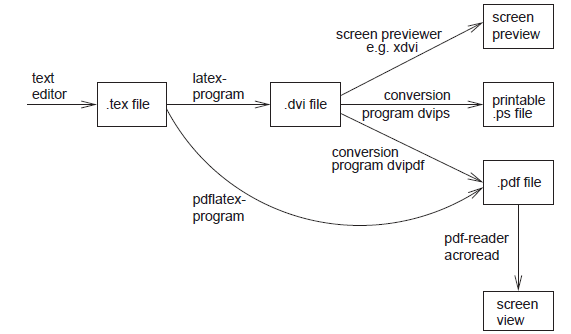
\includegraphics[scale=0.45]{images/latexhowthis}
   	\end{figure}
   \end{frame}
   
   
   
   \begin{frame}[<+->]{Installation}
   	\textbf{First you need a TEX Distribution:} contains all the software that you need to create a LATEX document.
   	\begin{itemize}
   		\item \href{http://miktex.org/}{MiKTeX}: A a free TeX distribution for Windows systems.
   		\item \href{http://www.tug.org/mactex/}{MacTeX}: A a free TeX distribution for Mac.
   		\item \href{https://www.tug.org/texlive/}{TeXLive}: A a free TeX distribution for for most flavors of Unix and windows.
   		\item  For more Latex info: https://www.latex-project.org/
   	\end{itemize}
   	
   \end{frame}
   
   
   \begin{frame}[<+->]{Installation}
   	\textbf{You also need a text editor:} To create a LATEX source file
   	\begin{itemize}
   		\item \href{http://www.xm1math.net/texmaker/}{Texmaker}.
   		\item \href{http://www.texstudio.org/}{TexStudio}.
   		\item We will use TexStudio with MiKTex
   		\begin{itemize}
   			\item Download \href{http://www.texstudio.org/}{TexStudio} for your distribution
   			\item Install TexStudio when MiKTeX installation is completed.
   			\item TexStudio will automatically configure the settings for you.
   		\end{itemize}
   		\item The installation of LaTeX is now complete.
   	\end{itemize}
   \end{frame}
   
   \begin{frame}[<+->]{Online versions}
   	Three popular online versions
   	\begin{itemize}
   		\item Overleaf [https://www.overleaf.com/].
   		\item Papeeria [https://papeeria.com/].
   		\item Sharelatex [https://www.sharelatex.com/].
   		\item Authorea [https://www.authorea.com/].
   	\end{itemize}
   \end{frame}

\section{Latex Command}

\begin{frame}[fragile]{Activity}
\begin{center}
	{\Large \textbf{Activity 1}}
\end{center}

\end{frame}

\begin{frame}{Commands}
	A LATEX document is mainly defined through commands. \\ 
Commands are case sensitive, and take one of the following two formats:
	\begin{itemize}
		\item They start with a backslash \alert{\textbackslash}  and then a name consisting of letters only.
		\item Some commands need an argument, which has to be given between curly braces \{  \}.
		\item Some commands support optional parameters, which
		are added in square brackets [ ].
	\end{itemize}
\end{frame}



\begin{frame}[fragile]{Commands}
	\framesubtitle{Arguments and Options}
	\begin{itemize}
		\item Many commands require a single argument, and some commands require even multiple arguments.
		\item Some commands can have several options.
	\end{itemize}
	\alert{Example:}
	\begin{minted}{tex}
	\usepackage{graphicx} % single argument
	\usepackage{amsmath, amssymb} % multiple arguments
	\documentclass[a4paper,11pt]{article} % several options
	\usepackage[final]{microtype}  % single options
	\end{minted}
\end{frame}


\begin{frame}[fragile]{Commands}
	\framesubtitle{Environment}
An environment is be marked by, \mintinline{tex}{\begin{environment} ... \end{environment}}.

\begin{itemize}
	\item These initiate and exit an environment.
	\item The type of environment is applied to everything between the begin and end commands.
\end{itemize}
\alert{Example:}
\begin{minted}{tex}
\begin{document}
content...           % document environment
\end{document}
\end{minted}
\end{frame}


\begin{frame}{Special Character}
	There are ten characters which, like the backslash, are used by latex for special purposes.\\
	\begin{figure}
  	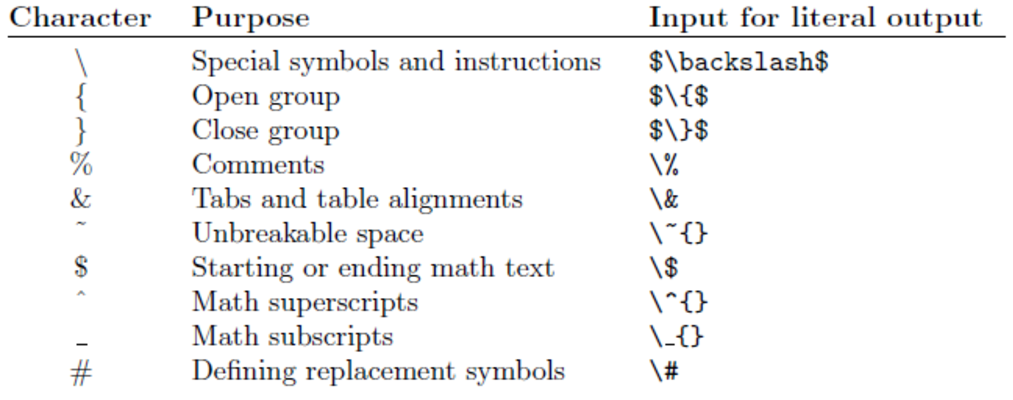
\includegraphics[scale=0.65]{images/special.pdf} 
	\end{figure}

\end{frame}

\section{Document Structure}



\begin{frame}[fragile]{Document Structure}
	Every LaTeX document has the following form:
	\begin{minted}{tex}
	\documentclass[options]{class name}
	
	%Preamble
	
	\begin{document}
	
	%Body
	
	\end{document}
	\end{minted}
	
\end{frame}



\begin{frame}[fragile]{Document Class}
	\begin{itemize}
		\item The command \mintinline{tex}{\documentclass[options]{class name}}  specify type of document you wants to create.
		\begin{itemize}
			\item \textbf{class name}: specifies the type of document to be created.
			\item \textbf{options parameter}:customises the behaviour of the document class.\\
		\alert{	Example:} 
		\mint{latex}{\documentclass[11pt,a4paper]{article}}	
 
			
			
		
		\end{itemize}
	\end{itemize}
\end{frame}


\begin{frame}{Document Class}
	Lists of the
	document classes type.\\
	\centering
	\scalebox{0.8}{
		\begin{tabular}{lp{12cm}}  
			\toprule
			\textbf{Class}    & \textbf{Description} \\
			\midrule
			article  & For articles in scientific journals, presentations, short reports, program documentation, invitations etc. \\
			report & For longer reports containing several chapters, small books, thesis etc.\\
			book & For real books.\\
			letter & For writing letters.\\
			beamer & For writing presentation\\
			exam  & For writing exams.\\
			\bottomrule
		\end{tabular}%
	}
	\label{tab:class1}%
	\vspace{1.5in}
\end{frame}



\begin{frame}{Document Class: Options}
 The
	document classes options.
	\centering
	\scalebox{0.8}{
		\begin{tabular}{lp{10cm}}  
			\toprule
			\textbf{Options}    & \textbf{Description} \\
			\midrule
			10pt, 11pt, 12pt  & Sets the size of the main font in the document. Default is 10pt. \\
			a4paper,letterpaper.. & Defines the paper size.The default size is
			letterpaper.Besides that, a5paper, b5paper, executivepaper,
			and legalpaper can be specified.\\
			twocolumn & Instructs LaTeX to typeset the document in two columns instead of one.\\
			twoside, oneside & For writing letters.\\
			landscape & Changes the layout of the document to print in landscape mode.\\
			titlepage, notitlepage & Specifies whether a new page should be started
			after the document title or not. The article class does not start a
			new page by default, while report and book do.\\
			\bottomrule
		\end{tabular}%
	}
	\label{tab:option}%
	
\end{frame}

\defverbatim[colored]\sleepSort{
	\begin{lstlisting}[language=TEX,tabsize=1]
	\documentclass[options]{class name}
	
	%Preamble
	
	\begin{document}
	\end{lstlisting}}

\begin{frame}[fragile]{Activity}
	\begin{center}
		{\Large \textbf{Activity 2}}
	\end{center}
	
\end{frame}

\begin{frame}[fragile]{The Preamble}
	The preamble is where you define the style of your document
	and load any packages you need to use.
     \begin{minted}{tex}
     \documentclass[options]{class name}
     
     %Preamble
     
     \begin{document}
     \end{minted}
		 
		\begin{itemize}
			\item It normally contains commands, variables or other things needed that affect the entire document.
			\item Load needed packages along with any options for those packages.
		\end{itemize}
	
\end{frame}


\begin{frame}[fragile]{The Preamble}
	The preamble is also used to load any other options or information
	that isn't necessarily a part of the document's content such as:
	\begin{itemize}
		\item Setting lengths of spaces before/after paragraphs, line height, etc
		\item Specifying author/title/date, etc. (important if you will be making a title
		page).
	\end{itemize}

\end{frame}


\begin{frame}[fragile]{The Preamble}
	\framesubtitle{Document Tittle}
	There are two steps to give your document a title.
	\begin{itemize}
		\item Tell LaTeX what to put in the title, and tell LaTeX to typeset the title.
		\item 	To specify title use the following commands in preamble:
		\mintinline{tex}{\title{...}, \author{...}, \date{..}}.
		\item  To display the title, use \mintinline{tex}{\maketitle} just after \mintinline{tex}{\begin{document}}.
	\end{itemize}
	\alert{Example:}
	\begin{minted}{tex}
        \title{Scintific Writing using LaTeX}
        \author{M.~Chuwa \and S.~Nyondo}
        \date{\today}
	\end{minted}
\end{frame}

	

\begin{frame}[fragile]{The Preamble: Packages}
	Packages extend the basic LATEX commands.
	\begin{itemize}
		\item To use packages, include the following  command:\mint{tex}|\usepackage[options]{package}|
		\item This command goes into the preamble of the document.
	\end{itemize}
  \alert{Example:}
  \begin{minted}{tex}
%To set margin
\usepackage[top=2in,bottom=1in,left=1in,right=1in]{geometry}  
\usepackage{microtype} %improves the spacing between words and letters
\usepackage{amsmath} %introduces several improvements for math environments
\usepackage{graphicx} % for inserting image in latex document
  \end{minted}
\end{frame}

\begin{frame}[fragile]{Activity}
	\begin{center}
		{\Large \textbf{Activity 3}}
	\end{center}
	
\end{frame}

\begin{frame}{The Body of the Document}
	After the preamble comes the \alert{body}.
	\begin{itemize}
		\item Starts with \mintinline{tex}{\begin{document}} and ends with \mintinline{tex}{\end{document}}
		\item This is where you fill in the actual content of your document.
		\item Contains all text, fgures, tables, etc.
	\end{itemize}
\end{frame}


\begin{frame}{The Body of the Document}
	You can organize your document using the following commands.
	\begin{figure}
		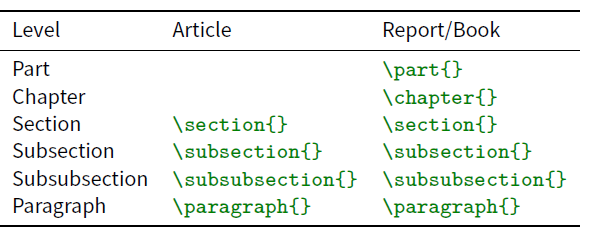
\includegraphics[scale=0.45]{images/structure}
	\end{figure}
	\begin{itemize}
		\item Your PDF output will include these sections as bookmarks.
		\item The above commands have a *-version and using these results in no number
		and no entry in the table of contents.
		\item Example: \; \mintinline{tex}{\subsection*{Acknowledgement}}
	\end{itemize}
\end{frame}


\begin{frame}[fragile]{Activity}
	\begin{center}
		{\Large \textbf{Activity 4}}
	\end{center}
	
\end{frame}



\section{Text Formatting}
\begin{frame}{Font Sizes and Colors}
	To change the font size in LaTeX \\
	\begin{table}[]
		\begin{tabular}{ll}  
			\toprule
			\textbf{Commands}    & \textbf{Output} \\
			\midrule
			\mintinline{tex}{\tiny} & \tiny{LaTex}\\
			\mintinline{tex}{\small} & \small{LaTex}\\
			\mintinline{tex}{\normalsize} & {\normalsize LaTex}\\
			\mintinline{tex}{\large} & \large{LaTex}\\
			\mintinline{tex}{\Large} & \Large{LaTex}\\
			\mintinline{tex}{\LARGE} & \LARGE{LaTex}\\
			\mintinline{tex}{\huge} & {\huge LaTex}\\
			\mintinline{tex}{\Huge} & \Huge {LaTex}\\
			\bottomrule
		\end{tabular}%
		\label{tab:size}%
	\end{table}
\end{frame}


\begin{frame}{Font Sizes and Colors}
To change text color use \mintinline{tex}{\usepackage{color}} or  \mintinline{tex}{\usepackage{xcolor}}
\begin{itemize}
	\item command:  \mintinline{tex}{\textcolor{color}{text}}
	\item Example: 
	\begin{itemize}
		\item \mintinline{tex}{\textcolor{red}{Hello} world} $\Rightarrow$ \textcolor{red}{Hello} world
		\item \mintinline{tex}{Hello \textcolor{blue}{world}} $\Rightarrow$ Hello \textcolor{blue}{world}
	\end{itemize}
	
\end{itemize}	

\end{frame}

\begin{frame}{Font Types and Style }
	To change the font itself to different styles
	\begin{table}[]
		\begin{tabular}{lll}  
			\toprule
			\textbf{Style} &\textbf{Commands}  & \textbf{Output} \\
			\midrule
			Bold & \mintinline{tex}{\textbf{LaTex}} & \textbf{LaTex}\\
			Italic &	\mintinline{tex}{\textit{LaTex}} & \textit{LaTex}\\
			Underline & \mintinline{tex}{\underline{LaTex}} & \underline{LaTex}\\
			Typewriter &	\mintinline{tex}{\texttt{LaTex}} & \texttt{LaTex}\\
			Sans-Serif & \mintinline{tex}{\textsf{LaTex}} & \textsf{LaTex}\\
			Serif (Roman) &	\mintinline{tex}{\textrm{LaTex}} & \textrm{LaTex}\\
			\bottomrule
		\end{tabular}%
		\label{tab:size}%
	\end{table}
	
\end{frame}


\begin{frame}{Spacing}
	LaTex treats any number of spaces as a single space.
	\begin{itemize}
		\item Single new lines are treated as if there is no new line.
		\item Multiple blank lines are treated as a single new line or you may use \mintinline{tex}{\newline} command.
		\item You can force horizontal and vertical space using the \mintinline{tex}{\hspace{length}} and \mintinline{tex}{\vspace{length}}
		\begin{itemize}
			\item You have to give each command a length commands:
		\end{itemize} \mintinline{tex}{\hspace{0.1cm}},\\ \mintinline{tex}{\hspace{1in}} or\\ 
		\mintinline{tex}{\hspace{10pt}}
		
	\end{itemize}
\end{frame}



\begin{frame}[fragile]{Lists}
There are three list environments
\begin{itemize}
	\item itemize $\Rightarrow$ for a bullet list.
	\item enumerate $\Rightarrow$ for an ordered list and
	\item description $\Rightarrow$ for a descriptive list.
\end{itemize}
All lists follow the following format:
\begin{minted}{tex}
\begin{list_type}  
\item The first item 
\item The second item 
\item The third etc 
\end{list_type}
\end{minted}
\end{frame}

\begin{frame}[fragile]{Lists}
	\begin{columns}[c] % the "c" option specifies center vertical alignment
		\column{.5\textwidth} % column designated by a command
		\begin{minted}{tex}
\begin{itemize}
\item The first item
\item The second item
\item  The third item
\end{itemize}
		\end{minted}
		\column{.5\textwidth}
		\begin{itemize}
			\item The first item
			\item The second item
			\item  The third item
		\end{itemize}
	\end{columns}
\end{frame}

\begin{frame}[fragile]{Lists}
	\begin{columns}[c] % the "c" option specifies center vertical alignment
		\column{.5\textwidth} % column designated by a command
		\begin{minted}{tex}
	\begin{enumerate}
	\item The first item
	\item The second item
	\item The third item
	\end{enumerate}
		\end{minted}
		\column{.5\textwidth}
		\begin{enumerate}
			\item The first item
			\item The second item
			\item The third item
		\end{enumerate}
	\end{columns}
\end{frame}

\begin{frame}[fragile]{Lists}
The description list used to explain notations or terms
\begin{minted}{tex}
\begin{description}
\item[Itemize] used for a bullet list.
\item[Enumerate] used for a ordered list.
\item[Description] used for a descriptive list.
\end{description}
\end{minted}
\alert{output}
\begin{description}
\item[Itemize] used for a bullet list.
\item[Enumerate] used for a ordered list.
\item[Description] used for a descriptive list.
	\end{description}
	
\end{frame}


\begin{frame}[fragile]{Nested Lists}
	\begin{columns}[c] % the "c" option specifies center vertical alignment
		\column{.5\textwidth} % column designated by a command
\begin{minted}{tex}
\begin{enumerate}
\item Item one
   \begin{enumerate}
     \item Subitem one
     \item Subitem two
   \end{enumerate}
\item Item two
\end{enumerate}
\end{minted}
		\column{.5\textwidth}
		\begin{enumerate}
			\item Item one
			\begin{enumerate}
				\item Subitem one
				\item Subitem two
			\end{enumerate}
			\item Item two
		\end{enumerate}
	\end{columns}
\end{frame}


\begin{frame}[fragile]{Activity}
	\begin{center}
		{\Large \textbf{Activity 6}}
	\end{center}
	
\end{frame}

\section{Cross-reference}\label{cross-ref}

\begin{frame}[fragile]{Cross-reference}
With the commands \mintinline{tex}{\label{key}  and \ref{key}} it is possible to refer to section numbers.
\begin{itemize}
	\item The command \mintinline{tex}{\label{key}} is used to set an identifier that is later used in the command \mintinline{tex}{\ref{key}} to set the reference.
\end{itemize}

\alert{Example}:\\
Create label: \framebox[1.0\width]{\mintinline{tex}{\section{Cross-Reference}\label{cross-ref}}}\\

Reference:
\framebox[1.0\width]{\mintinline{tex}{It is not difficult to refer to Section \ref{cross-ref}}}\\

Output: \framebox[1.2\width]{It is not difficult to refer to Section \ref{cross-ref}}
\end{frame}

\begin{frame}[fragile]{Activity}
	\begin{center}
		{\Large \textbf{Activity 6}}
	\end{center}
	
\end{frame}

\section{Typesetting Mathematics}

\begin{frame}[fragile]{Math  mode}
The \texttt{amsmath} package is the backbone of using LaTex for typesetting math.
\begin{itemize}
	\item Include in preamble: \mintinline{tex}{\usepackage{amsmath}}
\end{itemize}
The math environment" comes in two different forms:
\begin{description}
	\item[Inline mode] $\Rightarrow$ format the math within existing lines of text.
	\item[Display mode] $\Rightarrow$ sets the math apart and centers it on the page.
\end{description}
\end{frame}

\begin{frame}[fragile]{Math  mode}
	\framesubtitle{Inline mode}
	Several options exist:
	\begin{itemize}
		\item Use:\mintinline{tex}{\begin{math} x + y = 2 \end{math}} $\Rightarrow$ \begin{math} x + y = 2 \end{math}
		\item Surround the math with \mintinline{tex}{\(x+y = 2\)}  $\Rightarrow$ \begin{math} x + y = 2 \end{math}
		\item Surround the math with single dollar signs \mintinline{tex}{$x + y =2$} $\Rightarrow$ $x + y = 2$
	\end{itemize}
\end{frame}

\begin{frame}[fragile]{Math  mode}
	\framesubtitle{Inline mode}
	Subscripts and superscripts in math mode are formed using the \mintinline{tex}{_} and the \mintinline{tex}{^}.\\
	\alert{Example:}
	\begin{center}
\framebox[1.1\width]{$a_n = n^2 + 1$} $\Rightarrow$  \framebox[1.1\width]{\mintinline{tex}{$a_n = n^2 + 1$}}
	\end{center}
	
	When the subscript or superscript is more than one character,
	you must wrap it in \{...\} to group it together.\\
	\alert{Example:} 
	\begin{center}
\framebox[1.1\width]{\(y_{n + 1} = e^{n^2-1} + 1\) } $\Rightarrow$  \framebox[1.1\width]{\mintinline{tex}{$y_{n + 1} = e^{n^2-1} + 1$}}
	\end{center}
\end{frame}

\begin{frame}[fragile]{Math  mode}
	\framesubtitle{Inline mode}
	Some common math symbols:
	\centering
	\scalebox{0.8}{
		\begin{tabular}{lp{5cm}}  
			\toprule
			\textbf{Symbol}    & \textbf{Output} \\
			\midrule
			\mintinline{tex}{\alpha,\beta,\lambda,\gamma,\theta,\mu etc} & $\alpha, \beta, \lambda, \gamma, \theta, \mu, $ etc \\
			\mintinline{tex}{\infty,\exists,\forall,\pm,\leq,\geq etc}. & $\infty,\exists,\forall,\pm,\leq,\geq$ etc\\
			\mintinline{tex}{\int_0^{\infinity},\sum_{i=1}^n,\prod_{n=1}^N } &  $\int_0^{\infty}, \sum_{i=1}^n, \prod_{n=1}^N$ etc\\
			\mintinline{tex}{\ldots, \cdots,\vdots,\colon etc} & $\ldots, \cdots,\vdots,\colon$etc \\
			\mintinline{tex}{\frac{x}{y}, \sqrt{x},\bar{x},\lim_{x \to \infty}} & $\frac{x}{y}, \sqrt{x},\bar{x}, \lim_{x \to \infty}$ etc\\
			\bottomrule
		\end{tabular}%
	}
	\label{tab:mathsymbol}%
	
\alert{More math symbols and formulas}: \href{https://en.wikibooks.org/wiki/LaTeX/Mathematics}{Latex Symbols} 
\end{frame}

\begin{frame}[fragile]{Math  mode}\framesubtitle{Common Math Formula}
	\framebox[1.2\width]{$\frac{\partial y}{\partial x}$} $\Rightarrow$  \framebox[1.1\width]{\mintinline{tex}{$\frac{\partial y}{\partial x}$}}\\
	
		\framebox[1.2\width]{$ \int_a^b f(x)\,dx $ } $\Rightarrow$  \framebox[1.1\width]{\mintinline{tex}{$ \int_a^b f(x)\,dx $ }}
\end{frame}

\begin{frame}[fragile]{Math  mode}
	\framesubtitle{Display mode}
	Several options exist:
	\begin{itemize}
		\item Using \mintinline{tex}{\begin{displaymath} x + y = 2 \end{displaymath}} $\Rightarrow$ \begin{displaymath} x + y = 2 \end{displaymath}
		\item Surround the math with \mintinline{tex}{\[x+y = 2\]}  $\Rightarrow$ \[ x + y = 2 \]
		\item Surround the math with double dollar signs \mintinline{tex}{$$x + y =2$$} $\Rightarrow$ $$x + y = 2$$
	\end{itemize}
\end{frame}

\begin{frame}[fragile]{Math  mode}
	\framesubtitle{Numbered Equation}
The \texttt{equation} environment: \mintinline{tex}{\begin{equation}...\end{equation}} creates a displayed formula and automatically generates
an equation number.\\
\alert{Example:}
\begin{equation}\int_{0}^{\pi}\sin x \,dx = 2\end{equation}
 \begin{center}$\Downarrow$\end{center} 
\mint{tex}{\begin{equation}\int_{0}^{\pi}\sin x \,dx = 2\end{equation}} 
\end{frame}

 \begin{frame}[fragile]{Math mode}
	\framesubtitle{Referencing equations}
	The amsmath package provides \mintinline{tex}{\eqref{key}} for referencing equations.\\
	\alert{Example:}
\begin{columns}
\begin{column}{0.5\textwidth}
	\begin{equation} \label{eq:1} 
	\sum_{i=0}^{\infty} a_i x^i 
	\end{equation}
	The equation \ref{eq:1} is a typical power series.
\end{column}
\hspace{5pt}\vrule\hspace{5pt}%
\begin{column}{0.5\textwidth}		
\begin{minted}{tex}
\begin{equation} \label{eq:1} 
\sum_{i=0}^{\infty} a_i x^i 
\end{equation}
The equation \ref{eq:1} is a typical power series.
\end{minted}
\end{column}
\end{columns}	
\end{frame}

\begin{frame}[fragile]{Activity}
	\begin{center}
		{\Large \textbf{Activity 7}}
	\end{center}
	
\end{frame}



\begin{frame}[fragile]{Math  mode}
	\framesubtitle{Multiple Equations}
The \mintinline{tex}{\begin{align}..\end{align}} environment is used group together several formulas or,  equations with more than one lines.
\alert{Example:}


\begin{columns}
	\begin{column}{0.5\textwidth}
		 \begin{align}
		\alpha + \beta^2 &= 0 \\
		\log_{10}2\alpha &=e^{\beta}-1
		\end{align}
	\end{column}
	\hspace{5pt}\vrule\hspace{5pt}%
	\begin{column}{0.5\textwidth}		
		\begin{minted}{tex}
\begin{align}
\alpha + \beta^2 &= 0 \\
\log_{10}2\alpha &=e^{\beta}-1
\end{align}
		\end{minted}
	\end{column}
\end{columns}	


\end{frame}

\begin{frame}[fragile]{Math  mode}
	\framesubtitle{Multiple Equations}
	To align several formulas or equations with more than one lines.
	\alert{Example:}
	\begin{columns}
		\begin{column}{0.5\textwidth}
				\begin{align*}
			y &=x^2 + 2x -1\\
			&=(x+1)(2x+1) \\
			&=(x+1)^2
			\end{align*}
		\end{column}
		\hspace{5pt}\vrule\hspace{5pt}%
		\begin{column}{0.5\textwidth}		
\begin{minted}{tex}
\begin{align*}
y &=x^2 + 2x -1\\
&=(x+1)(2x+1) \\
&=(x+1)^2
\end{align*}
			\end{minted}
		\end{column}
	\end{columns}	

	
\end{frame}



\begin{frame}[fragile]{Math  mode}
	\framesubtitle{Matrices and Array}
	A basic matrix may be created using the \texttt{matrix} environment.\\
	
\alert{Plain Matrix}
\begin{columns}
	\begin{column}{0.5\textwidth}
		\[
		\begin{matrix}
		\alpha& \beta^{*}\\
		\gamma^{*}& \delta
		\end{matrix}
		\]
	\end{column}
	\hspace{5pt}\vrule\hspace{5pt}%
	\begin{column}{0.5\textwidth}		
		\begin{minted}{tex}
\[
\begin{matrix}
\alpha& \beta^{*}\\
\gamma^{*}& \delta
\end{matrix}
\]
		\end{minted}
	\end{column}
\end{columns}	

\end{frame}


\begin{frame}[fragile]{Math  mode}
	\framesubtitle{Matrices and Array}

	\alert{Bracketed matrix}; typically represents the matrix itself\\
	
	\begin{columns}
		\begin{column}{0.5\textwidth}
			\[
			\begin{bmatrix}
			\alpha& \beta^{*}\\
			\gamma^{*}& \delta
			\end{bmatrix}
			\]
		\end{column}
		\hspace{5pt}\vrule\hspace{5pt}%
		\begin{column}{0.5\textwidth}		
			\begin{minted}{tex}
	\[
	\begin{bmatrix}
	\alpha& \beta^{*}
	\gamma^{*}& \delta
	\end{bmatrix}
	\]
			\end{minted}
		\end{column}
	\end{columns}	
		
\end{frame}


\begin{frame}[fragile]{Math  mode}
	\framesubtitle{Matrices}

	\alert{Parenthesized matrix}\\
	
	\begin{columns}
		\begin{column}{0.5\textwidth}	
			\[
		\begin{pmatrix}
		\alpha& \beta^{*}\\
		\gamma^{*}& \delta
		\end{pmatrix}
		\]
		\end{column}
	\hspace{5pt}\vrule\hspace{5pt}%
		\begin{column}{0.5\textwidth}
		
	\begin{minted}{tex}
\[
\begin{pmatrix}
\alpha& \beta^{*}\\
\gamma^{*}& \delta
\end{pmatrix}
\]
\end{minted}			
			
		\end{column}
	\end{columns}
\end{frame}

\begin{frame}[fragile]{Math mode}
	\framesubtitle{Matrix}
	\alert{Example: let type the following matrix}
	\[ A_{m,n} =
	\begin{pmatrix}
		a_{1,1} & a_{1,2} & \cdots & a_{1,n} \\
		a_{2,1} & a_{2,2} & \cdots & a_{2,n} \\
		\vdots  & \vdots  & \ddots & \vdots  \\
		a_{m,1} & a_{m,2} & \cdots & a_{m,n} 
	\end{pmatrix}
	\] 
	
\end{frame}


\begin{frame}[fragile]{Math mode}
	\framesubtitle{Matrix}
	\alert{Example: let type the following matrix}
	\begin{center}
\begin{minted}{tex}
\[
A_{m,n} =
\begin{pmatrix}
a_{1,1} & a_{1,2} & \cdots & a_{1,n} \\
a_{2,1} & a_{2,2} & \cdots & a_{2,n} \\
\vdots  & \vdots  & \ddots & \vdots  \\
a_{m,1} & a_{m,2} & \cdots & a_{m,n} 
\end{pmatrix}
\] 
\end{minted}
	\end{center}

	
\end{frame}

\begin{frame}[fragile]{Math mode}
	\framesubtitle{The Case Environment}
	The  \texttt{cases} environment allows the writing of piecewise functions.\\
	Consider the following:
	\begin{columns}
		\begin{column}{0.5\textwidth}	
\[
f(x) = 
\begin{cases} 
x & \text{if } x \neq 0 \\
\frac{\sin x}{x}       & \text{otherwise} 
\end{cases}
\]
\end{column}
	\hspace{5pt}\vrule\hspace{5pt}%
\begin{column}{0.5\textwidth}
\begin{minted}{tex}
\[
f(x) = 
\begin{cases} 
x & \text{if } x \neq 0 \\
\frac{\sin x}{x}& \text{otherwise} 
\end{cases}
\]
\end{minted}
\end{column}
\end{columns}	
\end{frame}

\begin{frame}[fragile]{Activity}
	\begin{center}
		{\Large \textbf{Activity 7}}
	\end{center}
	
\end{frame}

\section*{Code listing}

\begin{frame}[fragile]{Code listing}
	LaTeX allows formatting and highlighting source code in your documents.
	\begin{itemize}
		\item Several packages available: https://www.sharelatex.com/learn/Code\_listing
		\item Minted package  is pretty awesome and more powerful than the other  packages.
		\item  Minted uses the Python library Pygments
	\end{itemize}
\end{frame}


\begin{frame}[fragile]{Code listing}
	To use Minted \href{https://www.sharelatex.com/learn/Code_Highlighting_with_minted}{Minted}
	\begin{itemize}
		\item Load the minted package: \mintinline{tex}{\usepackage{minted}}
		\item In windows add the following line at the top of your tex file.
		% !TeX TXS-program:compile = txs:///pdflatex/[--shell-escape]
		\item  In-line listing: \mintinline{tex}{\mintinline{language}{code}}
		\item block listing: Use \mintinline{tex}{\begin{minted}{code}...\end{minted}} environment.
	\end{itemize}
\end{frame}

\begin{frame}[fragile]{Code listing}
	Example: Block-listing: $C++$
	\begin{minted}{cpp}
	#include<iostream>
	using namespace std;
	
	int main()
	{
	int num,factorial=1;
	cout<<" Enter Number To Find Its Factorial:  ";
	cin>>num;
	for(int a=1;a<=num;a++)
	{
	factorial=factorial*a;
	}
	cout<<"Factorial of Given Number is ="<<factorial<<endl;
	return 0;
	}
	\end{minted}
\end{frame}


\begin{frame}[fragile]{Code listing}
	Example: Python
	\begin{minted}{python}
	x = 2
	y = 3
	print{x + y}
	\end{minted}
	
	
\end{frame}



\section*{Collaborative Writing}
\begin{frame}[fragile]{Collaborative writing}
	Most of your writing will be collaborative:
	\begin{itemize}[<+>]
		\item often participants are distributed
		\item there are lots of ways to deal with this $\Rightarrow$ even when they are local, these techniques help.
		
	\end{itemize}
	
\end{frame}

\begin{frame}[<+>]{Collaborative writing}
	Available modes
	\begin{itemize}
		\item One person acts as editor, and incorporates changes: others  $\Rightarrow$ communicate proposed changes.
		\begin{itemize}
			\item [-] lots of work for editor, but only they end up happy.
		\end{itemize}
		\item Token: one person has the \alert{token} (for all or part)
		\begin{itemize}
			\item edit as please when have token pass it when $\Rightarrow$ finished (e.g. by email)
			\item [-] requires trust.
		\end{itemize}
		\item Truly distributed:
		\begin{itemize}
			\item [+] all have access, and can edit.
			\item [+] conflicts are merged
			\item [+-] very powerful, but requires tools.
		\end{itemize}
	\end{itemize}
\end{frame}


\begin{frame}[<+>]{Collaborative writing models
		Truly distributed collaboration}
	Require tools that support
	\begin{itemize}
		\item Distributed access { e.g. Dropbox} and Revision control
	\end{itemize}
	Available options:
	\begin{description}[Example]
		\item[Payfor] \href{https://www.overleaf.com/}{Overleaf}, \href{https://www.sharelatex.com/}{ShareLaTex}, \href{https://www.authorea.com/}{Authorea} and \href{https://papeeria.com/}{Papeeria}.
		\begin{itemize}
			\item [-] often have a free limited plan.
			\item [-] focussed on latex, not the rest (e.g. accompanying code and data).
		\end{itemize}
		\item [free: standard open source tools]  Version Control eg git
	\end{description}
	
\end{frame}

\begin{frame}[<+>]{Revision (or version) control}
	Features:\begin{itemize}
		\item Allow you to see all revisions of paper $\Rightarrow$ e.g. revert back to an old version if you don't like changes.
		\item Trace activity $\Rightarrow$ volume also what changed, with comments.
		\item Good for code,  LaTeX, and (some) data.
	\end{itemize}
	Cloud git services: \href{https://github.com/}{Github}, \href{https://bitbucket.org/}{BitBucket},\href{https://about.gitlab.com/}{Gitlab}.
\end{frame}


\begin{frame}
	\centering
	\Huge{THANK YOU}
\end{frame}

    \end{darkframes}
\end{document}
